\documentclass[12pt]{article}
\usepackage[papersize={70cm,100cm}]{geometry}
\usepackage{amsmath}
\usepackage[poster]{tcolorbox}
\pagestyle{empty}
\usepackage{multicol}
\usepackage{xcolor}
\usepackage[hidelinks]{hyperref}

% COLORES UTEC
\definecolor{azulutec}{HTML}{0D2875}
\definecolor{celesteutec}{HTML}{00ADEE}
\definecolor{negro}{HTML}{000000}
\definecolor{blanco}{HTML}{FFFFFF}

\begin{document}
\begin{tcbposter}[
        % opciones para los marcos
        poster={showframe=false, columns=4, rows=8,spacing=1.5mm},
        % fondo general blanco sin degradado
        coverage={spread, interior style={fill=blanco}},
        % estilo de cajas
        boxes={
                % sharp corners=downhill,
                arc=3mm,
                boxrule=1mm,
                colback=blanco,
                colframe=negro,
                title style={
                        left color=celesteutec,
                        right color=celesteutec
                    },
                fonttitle=\bfseries \Huge
            }
    ]

    % -------------------------------
    % TÍTULO
    % COLUMNA 1: Logo UTEC
    \posterbox[blankest,
        halign=center, valign=center,
        interior engine=path,
        interior style={fill=blanco}
    ]{name=logo,column=1,row=1}{
        
\includegraphics[height=9cm]{img/logoUTEC.png}
    }

    % -------------------------------
    % COLUMNAS 2–3: Título centrado
    \posterbox[blankest,
        halign=center, valign=center,
        fontupper=\bfseries\color{black}\huge,
        interior engine=path,
        interior style={fill=blanco}
    ]{name=titulo,column=2,row=1,span=2}{
        \begin{center}
            \resizebox{0.95\linewidth}{!}{\parbox{30cm}{\centering
                    “Optimización de filtros eléctricos en cargadores de baterías\\
                    para vehículos eléctricos mediante la aplicación de funciones de transferencia”
                }}\\[20mm]
            \resizebox{0.6\linewidth}{!}{\textbf{CURSO: ECUACIONES DIFERENCIALES ORDINARIAS}}
        \end{center}
    }

    % -------------------------------
    % COLUMNA 4: Lista de Integrantes
    \posterbox[blankest,
        halign=center, valign=center,
        fontupper=\bfseries\color{azulutec}\huge,
        interior engine=path,
        interior style={fill=blanco}
    ]{name=integrantes,column=4,row=1}{
        \begin{center}
            \textbf{Integrantes:}
            \begin{itemize}
                \item Choque Shuan Katherine Massiel
                \item Huamán Yay Alexis
                \item Oceda Chavez Elizabeth Emperatriz
                \item Vásquez Bustamante María Fernanda
            \end{itemize}
        \end{center}
    }

    % -------------------------------
    % INTRODUCCIÓN
    \posterbox[adjusted title=Introducción]{name=intro,column=1,row=2,span=2}{
        \huge
        El crecimiento de la movilidad eléctrica ha impulsado el desarrollo de tecnologías de carga más rápidas y eficientes. Sin embargo, uno de los principales desafíos es la presencia de distorsiones armónicas en la señal eléctrica, generadas por el uso de filtros tradicionales en los convertidores.

        Estas distorsiones afectan la eficiencia del proceso de carga y la vida útil de las baterías, provocando también pérdidas térmicas e inestabilidad en la red. Por ello, es necesario optimizar los filtros eléctricos utilizados en los cargadores.

        Este proyecto aplica funciones de transferencia como herramienta para modelar y mejorar el comportamiento dinámico del sistema de carga, con el objetivo de reducir la distorsión armónica, mejorar la estabilidad del sistema y elevar la calidad de energía suministrada al vehículo eléctrico.
    }



    % -------------------------------
    % OBJETIVOS
    \posterbox[adjusted title=Objetivos]{name=obj,column=1,row=3,rowspan=1,span=2}{
        \Huge
        \setlength{\columnsep}{1.5cm}
        \begin{multicols}{2}
            \textbf{Objetivo general:} \\

            Diseñar y optimizar filtros eléctricos aplicados en cargadores de baterías para vehículos eléctricos mediante funciones de transferencia, buscando mejorar la eficiencia energética, garantizar una salida estable y reducir la distorsión durante el proceso de carga.

            \columnbreak

            \textbf{Objetivos específicos:} \\

            Analizar el sistema con distintos filtrados ante señales alternas, evaluar la atenuación de armónicos mediante funciones de transferencia, comparar diseños convencionales y optimizados, y proponer un filtro robusto frente a perturbaciones.
        \end{multicols}
    }





    % -------------------------------
    % METODOLOGÍA
    \posterbox[adjusted title=Metodología]{name=metod,column=1,span=2,row=4, rowspan=5}{
        \centering
        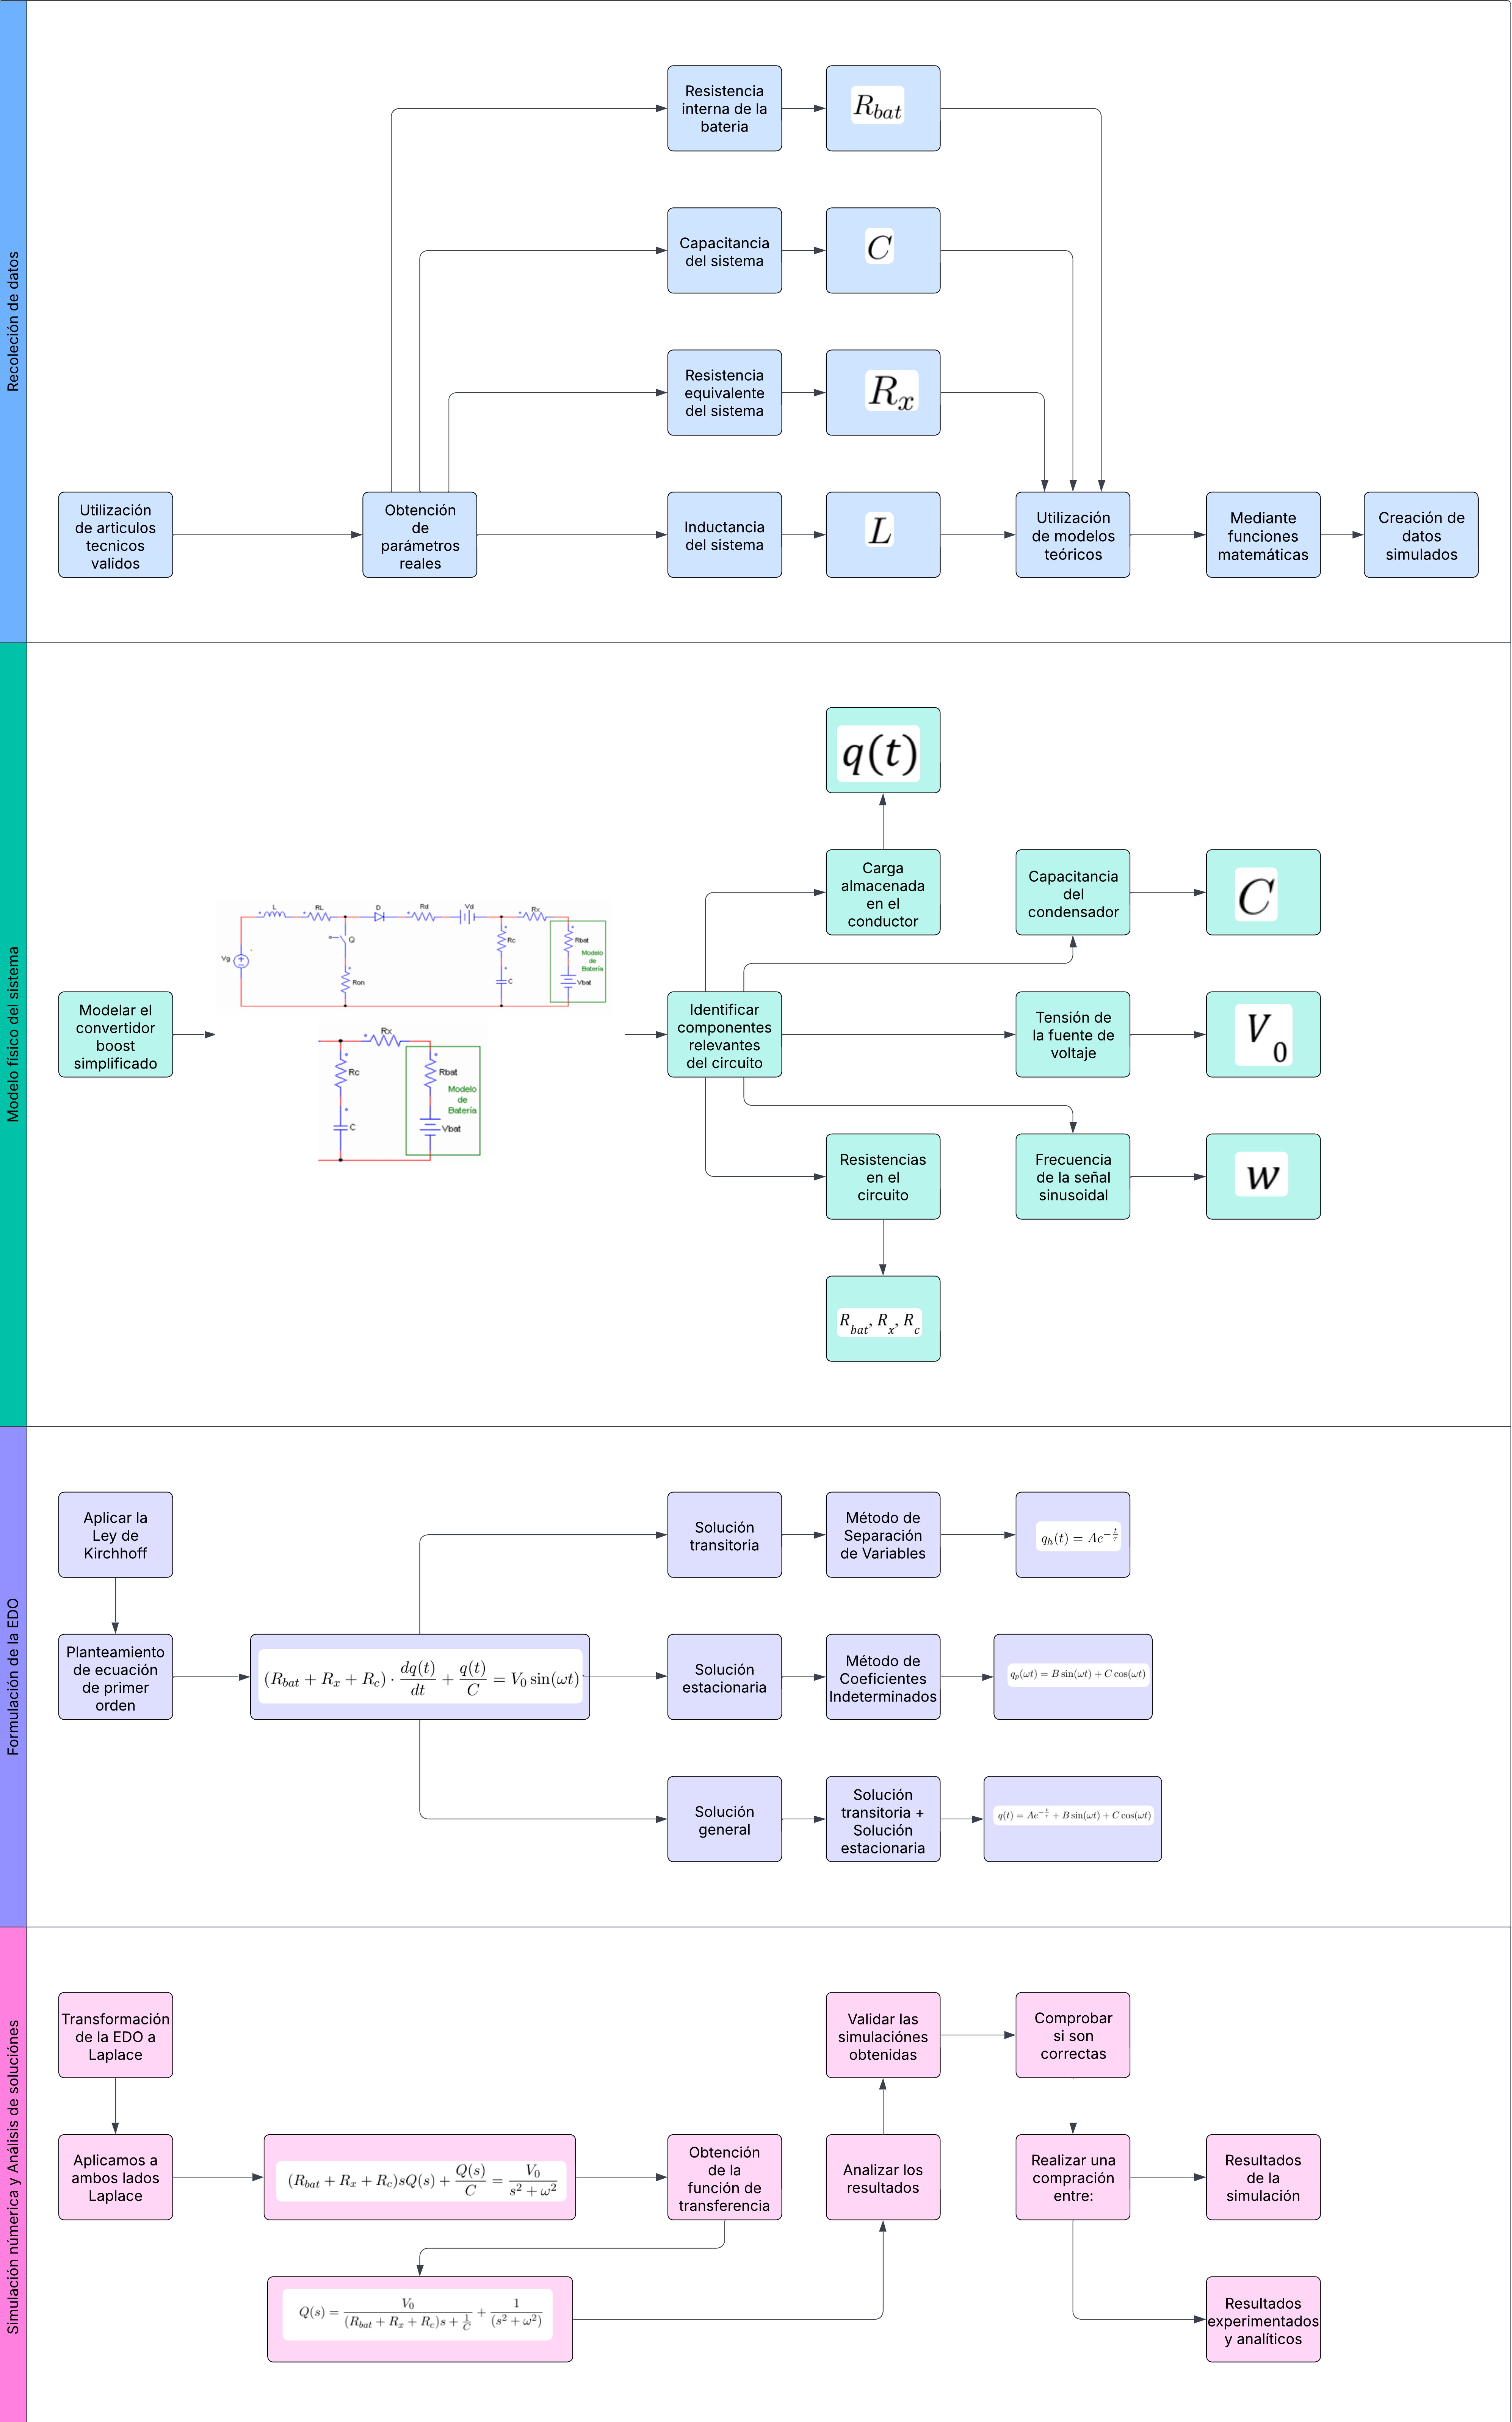
\includegraphics[width=\linewidth,height=1700pt]{img/diagrama.png}
    }


    % -------------------------------
    % RESULTADOS
    \posterbox[adjusted title=Resultados]{name=res,column=3,row=2,rowspan=4,span=2}{
        \huge
        Se estudió el comportamiento dinámico de un sistema de carga tipo RLC con señal senoidal, modelado mediante una EDO de primer orden. A partir de los parámetros obtenidos de la literatura, se planteó una ecuación diferencial que describe la evolución temporal de la carga en el condensador, y se resolvió analíticamente para obtener su solución general. Esta solución permitió identificar claramente las fases transitoria (decaimiento exponencial) y estacionaria (oscilación sinusoidal), ambas afectadas por el valor de la constante de tiempo \( \tau \) y la frecuencia de la señal de entrada \( \omega \).

        \vspace{2mm}

        Se empleó la función de transferencia y la transformada de Laplace como herramientas analíticas para resolver y modelar el sistema en el dominio de la frecuencia, facilitando su análisis frente a perturbaciones. Posteriormente, se realizaron simulaciones numéricas en Python, comparando la solución analítica con resultados computacionales, lo que permitió validar el modelo bajo condiciones realistas.

        \vspace{2mm}

        El análisis espectral mediante la FFT reveló una marcada reducción de armónicos superiores y un claro predominio de la frecuencia fundamental, lo cual confirma la efectividad del filtro en mejorar la calidad de la señal. Los parámetros utilizados fueron:

        \vspace{10mm}
        \begin{center}
            \renewcommand{\arraystretch}{1.5}
            \begin{tabular}{|c|c|c|l|}
                \hline
                \textbf{Parámetro} & \textbf{Valor}  & \textbf{Unidad} & \textbf{Fuente}           \\
                \hline
                $R_{bat}$          & 0.2             & $\Omega$        & Sainz y Balcells (2011)   \\
                $R_z$              & 0.1             & $\Omega$        & Cittanti et al. (2021)    \\
                $R_c$              & 0.3             & $\Omega$        & Asumido por diseño        \\
                $C$                & 1000            & $\mu F$         & Estándar de carga lenta   \\
                $\omega$           & $2\pi \cdot 60$ & rad/s           & Corriente alterna (60 Hz) \\
                \hline
            \end{tabular}
        \end{center}

        \vspace{10mm}

        \textbf{Hallazgos clave:}
        \begin{itemize}
            \item El sistema muestra estabilización rápida determinada por la constante de tiempo \( \tau \).
            \item El filtro optimizado atenúa armónicos no deseados y mejora la calidad de la señal.
            \item Las simulaciones en Python coinciden con la solución analítica, validando el modelo.
        \end{itemize}

        \vspace{10mm}

        \begin{minipage}[t]{0.49\textwidth}
            \centering
            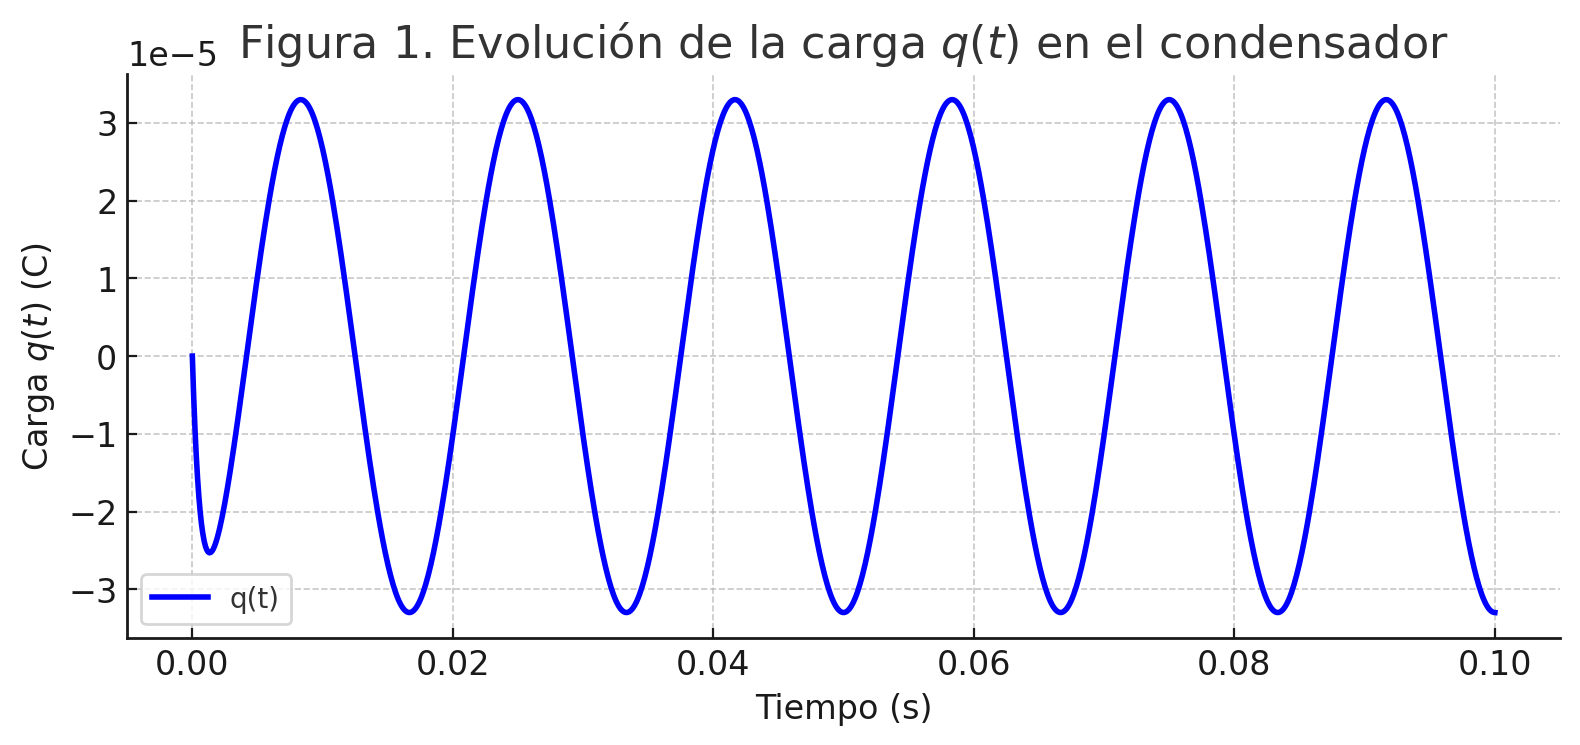
\includegraphics[width=\linewidth]{img/7.png}\\
            \textbf{Figura 1.} Carga del condensador \( q(t) \)
        \end{minipage}
        \hfill
        \begin{minipage}[t]{0.49\textwidth}
            \centering
            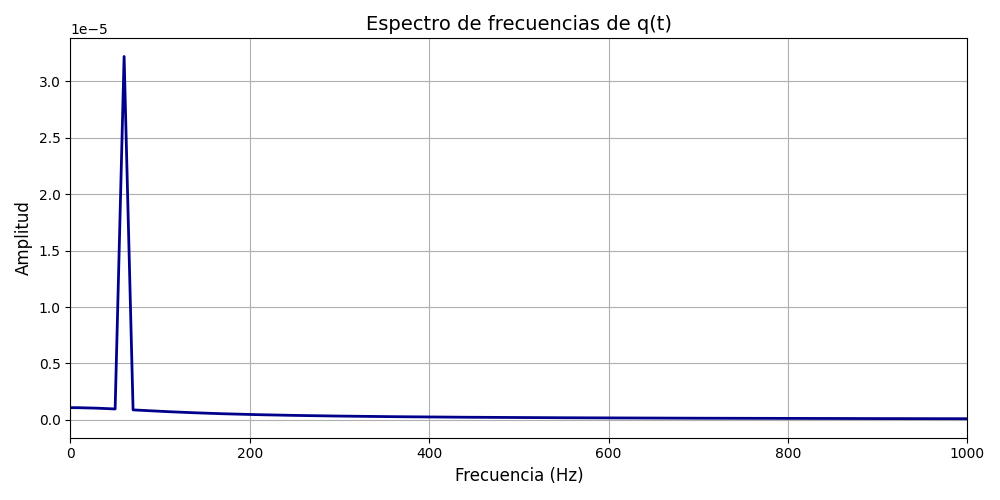
\includegraphics[width=\linewidth]{img/8.png}\\
            \textbf{Figura 2.} Espectro de frecuencias de \( q(t) \)
        \end{minipage}
    }


    % -------------------------------
    % CONCLUSIÓN
    \posterbox[adjusted title=Conclusión]{name=con,column=3,span=2,row=6,rowspan=2}{
        \huge
        \setlength{\columnsep}{1.5cm}
        \begin{multicols}{2}

            • \textbf{Resumen de los hallazgos principales:} \\
            El modelo propuesto permitió predecir con precisión el comportamiento dinámico del sistema de carga. Se comprobó que los filtros optimizados atenúan eficazmente los armónicos y mejoran la estabilidad y calidad de la señal, validando la función de transferencia como herramienta clave. Las simulaciones coincidieron con las soluciones analíticas, consolidando la validez del enfoque.

            \vspace{6mm}

            • \textbf{Relevancia teórica y práctica de los resultados:} \\
            El trabajo combinó teoría y práctica con éxito. Desde el enfoque teórico, se aplicaron herramientas matemáticas rigurosas como la transformada de Laplace y las leyes de Kirchhoff. En la práctica, los resultados impactan directamente en la eficiencia energética de los cargadores y en la vida útil de las baterías, permitiendo una mejor gestión de la energía.

            \columnbreak

            • \textbf{Relevancia para el campo de estudio:} \\
            Este estudio aporta al área de la electrónica de potencia, proponiendo mejoras concretas para los sistemas de carga. Su aplicación en movilidad eléctrica refuerza el valor del análisis matemático como base del diseño de tecnologías más confiables, limpias y sostenibles. También ofrece una guía para futuros desarrollos en filtros activos e híbridos.

            \vspace{6mm}

            • \textbf{Síntesis y relevancia del estudio:} \\
            En conjunto, se establece una base sólida para el desarrollo de filtros eficientes mediante el uso de EDOs. El enfoque analítico-simulativo demuestra que es posible diseñar soluciones robustas y validadas, destacando la importancia de las Ecuaciones Diferenciales en la ingeniería moderna. El trabajo muestra que la integración entre teoría, simulación y práctica genera propuestas aplicables en contextos reales de ingeniería eléctrica.

        \end{multicols}
    }


    % -------------------------------
    % BIBLIOGRAFÍA
    \posterbox[adjusted title=Bibliografía]{name=biblio,column=3,row=8,span=2}{
        \LARGE
        \textbullet\ Abundis, A. (2016). *Causas y efectos de armónicos en sistemas eléctricos de potencia*. Universidad Nacional Autónoma de México, Facultad de Ingeniería. \url{http://132.248.52.100:8080/xmlui/handle/132.248.52.100/11159}\par\medskip
        \textbullet\ Paipa, C. C., Ramirez, J. C., Trujillo R., C. L., Alarcón V., J. A., \& Jaramillo M., A. A. (2020). *Battery charger design with low current harmonic distortion for application in electric vehicles*. Ingeniare. Revista chilena de ingeniería, 28(4), 706–717. \url{https://dx.doi.org/10.4067/S0718-33052020000400706}\par\medskip
        \textbullet\ Cittanti, D., Mandrile, F., \& Bojoi, R. (2021). *Design Space Optimization of a Three-Phase LCL Filter for Electric Vehicle Ultra-Fast Battery Charging*. Energies, 14(5), 1303. \url{https://doi.org/10.3390/en14051303}
    }

\end{tcbposter}
\end{document}
